\documentclass[../Main.tex]{subfiles}
\begin{document}
\chapter{Algorithm Analysis}

\intro{

}

\section{Experimental Analysis}
\subsection{Drawbacks}
There are three major disadvantages when using experimental comparisons:
\begin{itemize}
    \item Experimental running times of two algorithms are difficult to directly compare unless the experiments are performed in the same hardware and software environments
    \item Experiments can be done only on a limited set of test inputs; hence, they leave out the running times of inputs not included in the experiment
    \item An algorithm must be fully implemented in order to execute it to study its running time experimentally
\end{itemize}

\begin{lstlisting}[language=Java, caption=Example Measurement]
    long startTime = System.currentTimeMillis();
    long endTime = System.currentTimeMillis();
    long elapsed = endTime - startTime;
\end{lstlisting}

\section{Growth Rates}
To analyze the runtime of algorithms without performing experiments, we perform an analysis directly on
a high level description of the algorithm.

\defn{Primitive Operations}{
    We define a set of primitive operations:
    \begin{itemize}
        \item Variable Assignment
        \item Reference Following
        \item Arithmetic Operation
        \item Comparison of two objects
        \item Accessing a single element of an array by index
        \item Method Calling 
    \end{itemize}
    Formally, a primitive operation corresponds to a instruction with an execution time that is constant.
}

\begin{figure}[H]
    \centering
    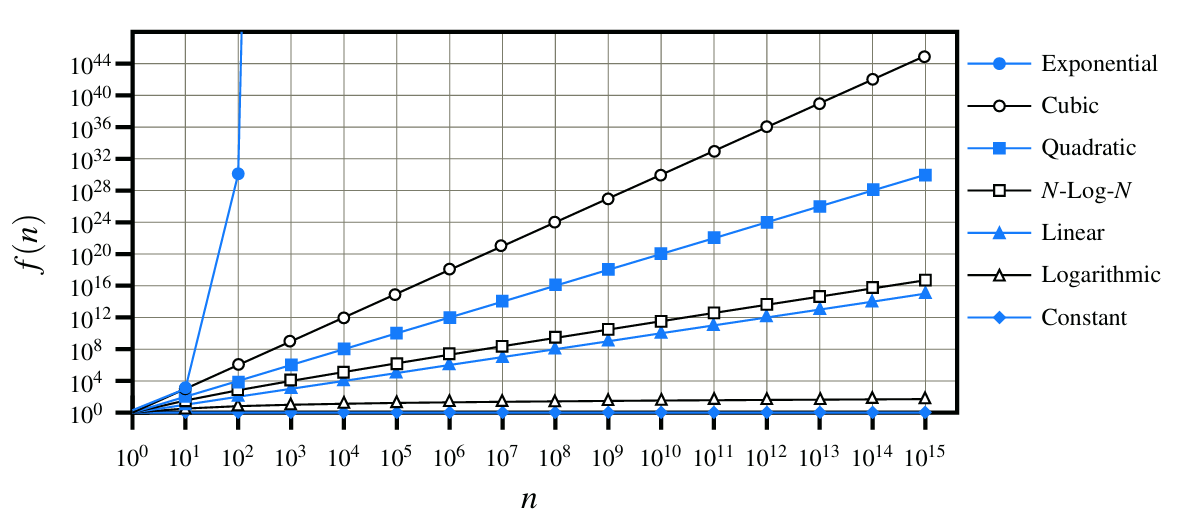
\includegraphics[width=1\linewidth]{Images/growthrates.png}
    \caption{Growth Rates for the seven fundamental functions on log-log. (exp with base a=2)}
\end{figure}
\newpage

\section{Asymptotic Analysis}
It is often enough to know that the running time of an algorithm grows proportionally to n.
Namely, we characterize the running times of algorithms
by using functions that map the size of the input, n, to values that correspond to
the main factor that determines the growth rate in terms of n.
\defn{Big-Oh}{
    Let \(f(n)\) and \(g(n)\) be functions,
    mapping positive integers to positive real numbers  \(\mathbb{N}^+ \rightarrow \mathbb{R}^+\).
    We say that \(f(n)\) is \(O(g(n))\) if there is a real constant \(c > 0 \) and an integer
    constant \(n_0 \leq 1\) such that:
    \begin{equation}
        f(n) \leq c \cdot g(n) \text{, for } n \geq n_0
    \end{equation}
}
We say: "\(f(n)\) is big-Oh of \(g(n)\)".
The big-Oh notation allows us to say that a function \(f(n)\) is “less than or equal
to” another function \(g(n)\) up to a constant factor and in the asymptotic sense as n
grows toward infinity. The big-Oh allows us to ignore constant factors and lower-order terms.
We should use the big-Oh notation to characterize a function as closely
as possible and describe the function in simplest terms.

Note that the use of the big-Oh and related notations can be somewhat misleading 
should the constant factors they “hide” be very large. 

\begin{figure}[H]
    \centering
    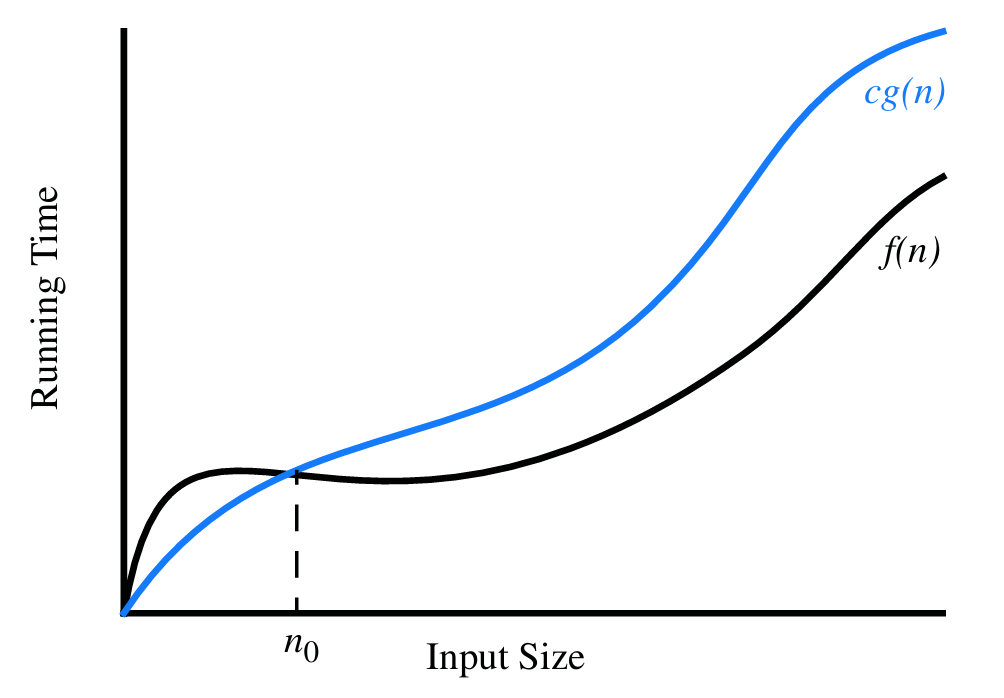
\includegraphics[width=0.75\linewidth]{Images/onotation.png}
    \caption{Big-Oh Notation}
\end{figure}




\defn{Polynomial big-Oh}{
    The highest-degree term in a polynomial is the term that determines the asymptotic 
    growth rate of that polynomial.
    \begin{equation}
        f(n)=a_0+a_1x+a_2x^2+\dots+a_dx^d \Rightarrow f(n) \in O(n^d)
    \end{equation}
    
}

\subsection{Other Notations}
\begin{itemize}
    \item Big-Omega lets us switch relations and expresses function growths greater than or equal to another.
    For this we say: "\(f(n)\) is \(\Omega(g(n))\)".
    \item Big-Theta allows to express that two functions grow at the same rate, up to constant factors.
    We say: "\(f(n)\) is \(\Theta(g(n))\)".
    \begin{equation}
        c'g(n) \leq f(n) \leq c''g(n) \text{, for } n \geq n_0
    \end{equation}
\end{itemize}

\end{document}
